%----------------------------------------------------------------------------
\chapter{The used cyberphysical system}
%----------------------------------------------------------------------------
\section{Usage of the designed software}

The designed monitoring software is made to be part of the system created for the Future Internet Research, Services and Technology project started by ETIK organization. The system is a prototype of a sensor network where the output of sensors can be used to create so called virtual sensors and store the data in a central data store. The system can reason using the ontology built on the sensors. A detailed introduction can be found in this chapter.

\section{Goal of the project}

The project's goal is to show a prototype of a cyberphisical system. It should contain sample sensors, a central database and also a planner, which plans the deployment of the designed new processes or virtual sensors. The system should prove using small example use cases that such a system is feasible to build. The prototype should not need to scale for large amount of sensors.

\section{System architecture}

The system was designed in the following way: 
There are computing or sensing resources called nodes which can provide computational capacity for the new application or sensor output using its sensors. The measurements are sent to the central SOS server and the available free resource information to the RDF store.
The SOS server stores the measurements and provide the data to the other nodes. There is a translation module, which can create the RDF representation of the sensor database for the ontology. 
The RDF store contains the overall architecture of the deployed applications and resource nodes. It also stores the load of each node. 
There is a sensor browser module which users can use to search in the ontology. It is connected to a measurement browser which will display the observations of the selected sensors. 
Users can deploy new application through the planner system. A package shall be uploaded and the planner should automatically deploy it to the chosen node. 
The status of the system can be seen on the implemented monitoring system.

\begin{figure}[h]
	\centering
	%custom
	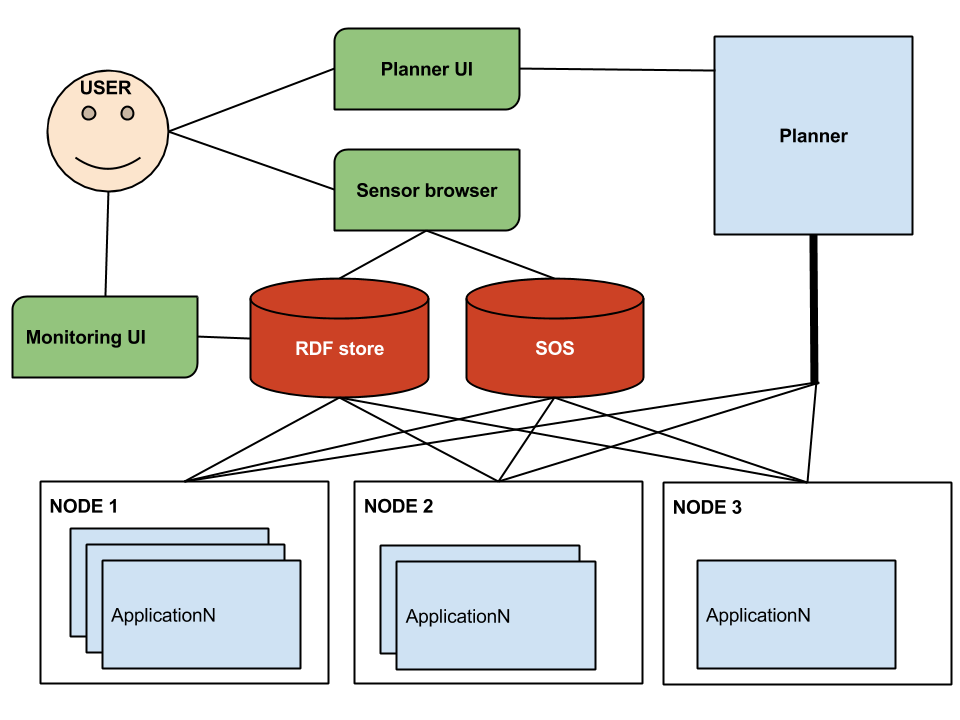
\includegraphics[width=0.6\textwidth]{figures/sysarch.png}
	\caption{System overview\label{fig:sysover}}
\end{figure}

\section{Sensors and resources}
The system is using different devices with different capabilities. There are simple microcontrollers and high performance mobile phones integrated in the system. 

The most simple solution is the Arduino Uno board with Ethernet controller. The card has an AVR based microcontroller working inside. It is good for simple measurement. It contains 14 general purpose inputs and outputs from which 6 can be PWM output. It's computing speed is 16Mhz.

The next in computational power is the Raspberry PI computer. This computer was designed to be cheap, reliable and compact, so poor people in developing countries can afford it. There are two models, both of them are fully working desktop computer with 700Mhz ARM cpu. It has:
\begin{itemize}
	\item 3 USB port
	\item 1 CSI port for raw camera input
	\item 1 Composite video output
	\item 1 HDMI output
	\item 1 SD/MMC/SDIO card reader
	\item 8 GPIO port (for UART, SPI, I2C, I2S audio)
\end{itemize} 
 It can run multiple operating systems, like Arch Linux, Raspbian OS, Debian, Slackware, etc. The more expensive model which costs around 35 dollars has a built in Ethernet port.  

The most expensive embedded computer is the BeagleBone in the project. This computer was developed by Texas instruments. It has a 600Mhz ARM Cortex 8 processor with 128 MB of RAM. It has built in features for sound and video processing. It costs around 150 USD. 

\section{The Sensor Observation Service}

The sensors communicate with the 52n SOS server using POX GET requests. To reach the service the sensors have to be in the same network or VPN to make the connection secure. The service has its own client installed next to it.

\section{RDF store}

The ontology is stored in an RDF database. It is based on the ontology introduced in the previous Chapter. The SSN Ontology has been extended for the custom use cases. The introduced ontology is called SISRO. It extends the original ontology in two ways:
\begin{itemize}
	\item It describes concepts and relations present in SensorML (and missing from SSN)
	\item It contains hardware details of the sensor devices
\end{itemize}


For easy communication with the sensors and the SOS server, the system can be reached using a custom service.
This Sensor Instance Semantic Registry Service contains the following interfaces:
\begin{itemize}
	\item Collection of Sensor Metadata. This interface contains the metadata for discovering sensors.
	\item System Discovery Interface. This interface is responsible for discovering sensors, searching in them using semantic connections.
	\item Sensor Status Interface. This interface manages the status information of the sensors. This interface makes it possible to search based on Status Information and change states.
	\item Sensor and hardware interconnection interface. Sensors does not have hardware description in SensorML. This interface supports application installation information and reconfiguration.
	\item SPARQL interface. This interface lets users to interact with the database on a low level.	  
\end{itemize}
The layer architecture can be seen on Figure \ref{fig:sisrserv}.	

\begin{figure}[h]
	\centering
	%custom
	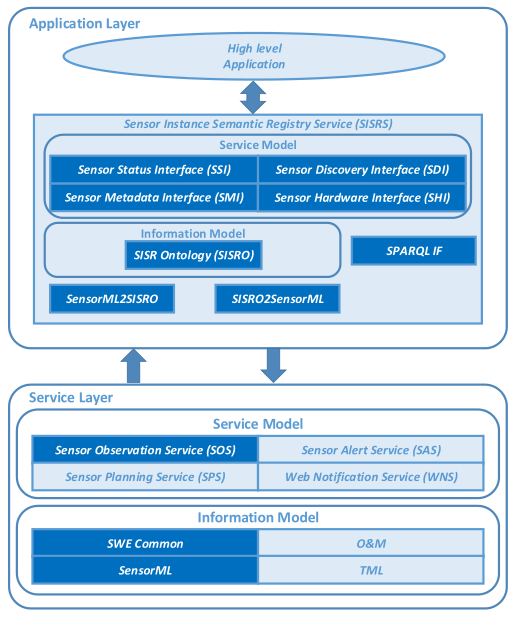
\includegraphics[width=0.6\textwidth]{figures/sisrserv.png}
	\caption{SISR service layers\label{fig:sisrserv}}
\end{figure}
The custom API has the following functions:
\begin{itemize}
\item GetCapabilities(): This function returns the sensor metadata from the database.
\item SearchSensor(): This function makes it possible to query the sensors based on temporal, spatial or topical properties.
\item DescribeSensor(): This function returns the SISRO ontology of a chosen sensor.
\item UpdateSensorInfo(): This function enables modification of sensor metadata.
\item GetSensorStatus(): This function retrieves sensor statuses.
\item SetSensorStatus(): This function lets the users modify sensor statuses.
\item AssignSensor(): This function assigns a sensor to a specific device.
\item RemoveSensor(): This function removes a sensor from the device.
\end{itemize}

\section{Planner}
The planer is a separate module that is capable of deploying different applications to the different resources. It is not used in the monitoring only its results, the deployed application.

\section{Image processing example application}

In the following example a a real life use case of the built cyberphisical system is solved. This example has been implemented in the project itself\cite{g6d1}. 

The goal was to check visual signals in a server room. There was a switch in the room what had blinking LED lights for indicating network connection. In this scenario we would like to monitor these connections only by using the LED indicators. The application is capturing a live video stream from the server room. In the video stream, the LEDs are seen. The user can specify the position of the monitored LEDs. The observations are categorized into 3 different categories:
\begin{itemize}
	\item Switched off - The LED hasn't been turned on since 5 seconds
	\item Blinking
	\item Turned on - The LED hasn't been turned off in the past 5 second
\end{itemize}

\begin{figure}[h]
	\centering
	%custom
	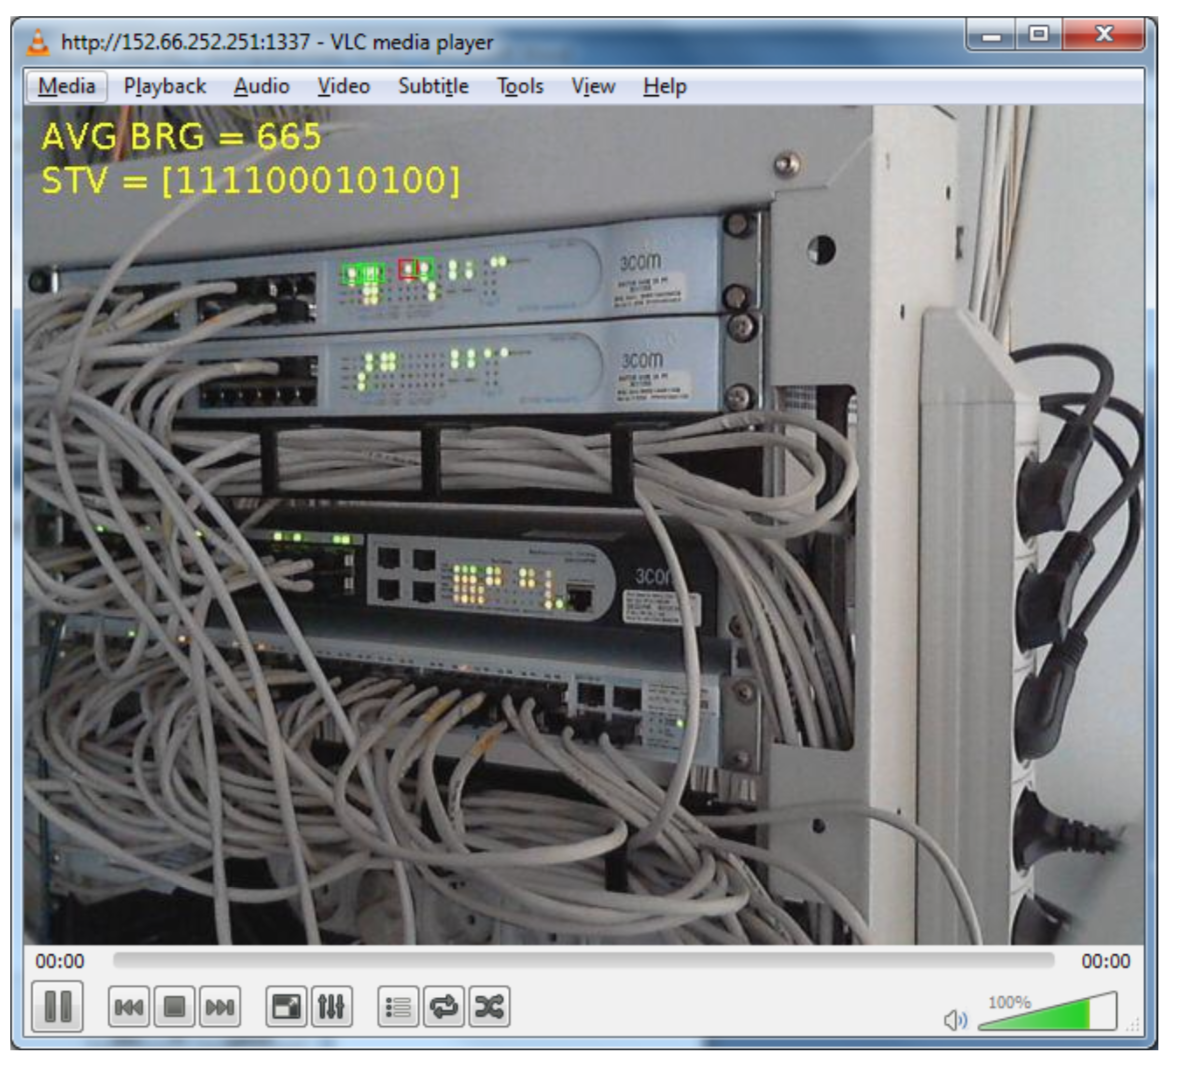
\includegraphics[width=0.6\textwidth]{figures/switchwork.png}
	\caption{Input image and corresponding output vectors\label{fig:switchwork}}
\end{figure}

The measurements are accumulated into a vector which projects each LED's state. Then the state vector is forwarded into the SOS database. The system also recognizes human interaction. If high movement is detected the system does not send the state vector but a marker signal that tells the system that human movement is detected. If there has been no movement for a long time, the system should automatically recover and show the state of the LEDs. The sensor input is stored in a plain text file.

The video capturing is done by a Raspberry PI device. The stream is sent to a Beagleboard computer which is running the the image processing application. It has the text file with the configuration. The text file contain 5 different lines:
\begin{itemize}
	\item[server] the URL of the video stream.
	\item[username] username for password protected streams.
	\item[password] password for the protected stream.
	\item[sos] URL for the POX endpoint of the SOS database.
	\item[point] there can be multiple of this descriptor, which sets the X and Y coordinates of the LEDs
\end{itemize}	
The input image and the output state vector can be seen on Figure \ref{fig:switchwork}.

\section{RDF representation of node load indicator}

As presented before the performance and load indicators are stored in the RDF store and the SOS server. The RDF store contains application and device descriptions too. Each node is uploading it's properties and applications to the store separately. The actual data is described in this section.

\subsection{Inserting Device description}


\begin{lstlisting}[caption={Template for Device information\label{lst:tempdev}}]
PREFIX rdf: <http://www.w3.org/1999/02/22-rdf-syntax-ns#>
PREFIX dedo: <http://purl.org/net/sisr/owl/dedo#>
PREFIX : <http://localhost:5820/sisro/data#>

# Inserting the device into the store
INSERT DATA
{ 
:DEVICEID rdf:type dedo:Device ;
rdf:type owl:NamedIndividual ;
dedo:device-type "DEVICETYPE"^^xsd:string .

:DEVICEIDHardware rdf:type dedo:Hardware ;
rdf:type owl:NamedIndividual ;
dedo:isPartOf :DEVICEID .

:DEVICEIDHardwareCPU rdf:type dedo:CPU ;
rdf:type dedo:NamedIndividual ;
dedo:isPartOf :DEVICEIDHardware ;
dedo:cpu-description "CPUDESCRIPTION"^^xsd:string ;
dedo:cpu-computing-power "MEEPS"^^xsd:double ;
dedo:cpu-computing-power-unit "MIPS"^^xsd:string .

:DEVICEIDHardwareMemory-RAM rdf:type dedo:OperationalMemory ;
rdf:type owl:NamedIndividual ;
dedo:isPartOf :DEVICEIDHardware ;
dedo:operational-memory-capacity "MEMORY"^^xsd:double ;
dedo:operational-memory-capacity-unit "MB"^^xsd:string .

:DEVICEIDHardwareMemory-Store rdf:type dedo:Storage ;
rdf:type owl:NamedIndividual ;
dedo:isPartOf :DEVICEIDHardware ;
dedo:storage-capacity "STORAGE"^^xsd:double ;
dedo:storage-capacity-unit "GB"^^xsd:string .
} 
\end{lstlisting}

